\begin{example}\label{ex:f_1}
Let $F_1$ be the free group on generators $x_1,x_2,x_3$ and $H_1$ its
subgroup $H_1=\la
h_1,h_2,h_3\ra$, where  $h_1= x_1^3$, $h_2=x_2x_3x_2^{-1}$ and
$h_3=x_1x_2x_3\ra$.

The Stallings automata, $\G_{A_1}$ for $H_1$,
with maximal subtree $T_1$ highlighted and base vertex $1$, is shown
in Figure \ref{fig:stall}.\ref{fig:stall1}.
The set $L_{T_1}$ corresponding to the maximal subtree  $T_1$ is
 $L_{T_1}=\{1,x_1,x_1^{-1},x_2,x_3^{-1} \}$.

Let the set of double coset representatives for $H_1$ be $S_1=S_1^{(1)}
\cup S_1^{(2)}$.
To find the double coset normal form for the element $f_1 =
x_2x_3^2x_2^{-1} x_1^4x_3^3x_1^{-2}x_3^{-1}x_2^{-1}x_1^{-1}$: in
the notation of Algorithm I, use
${A_1}$ to read off the maximal acceptable prefix $h=x_2x_3^2x_2^{-1} x_1^3
=h_2^2h_1$
of $f_1$; and
the maximal $L_{Q_1}$ prefix $p=x_1$ of the remaining part of $f_1$. Next
$q^{-1}=x_1x_2x_3x_1^2x_3^{-3}$, which has maximal acceptable prefix
$g=x_1x_2x_3$. The maximal $L_{Q_1}$-prefix of the remaining part of $q^{-1}$
is then $t=x_1^2$. Setting $e=x_3$,
\[f_1=h\circ p\circ e\circ t^{-1}\circ g^{-1}.\]
As $p$ is an $L_{T_1}$-prefix of $pq$ we have $y=p$. On the other hand
$t$ is not an $L_{T_1}$-prefix of $q^{-1}$ and $\t(t)=2$, so $z=w(2)=x_1^{-1}$.
Now set
\[s=p\circ e\circ z^{-1}=x_1x_3x_1^{-1}\in S_1^{(1)}.\]
Then, writing $h^\prime=gtz^{-1}=h_3h_1$, the normal form for $f_1$ is
\[f_1=hs(h^\prime)^{-1}=(h_2^{2}h_1) x_1x_3x_1^{-1} (h_1^{-1}h_3^{-1})\in H_1S_1^{(1)}H_1.\]

To find the double coset normal form for the element
$f_2=x_3^{-1}x_2^{-1}x_1^{-1}x_2x_3x_2^{-1}x_1^{-1}$: use
${A_1}$ to read off the maximal acceptable prefix $h=x_3^{-1}x_2^{-1}x_1^{-1}$
of $f_2$;

{\ef The maximal acceptable prefix $ h= h_3^{-1} h_2$. Further, $p
= x_1^{-1}$ and since $(2,1)$ represents itself, $a = h_3^{-1}
h_2$, $b=c = 1$ but anyway $f_2 = h_3^{-1} h_2  x_1^{-1}$.}

 and  the
maximal $L_{Q_1}$-prefix $p=x_2x_3$ of the rest of $f_2$.  Next
$q^{-1}=x_1x_2$, which is readable by ${A_1}$, so
$t=q^{-1}=x_1x_2$ and
\[f_2=h\circ p\circ t^{-1}.\]
Therefore $f_2$ will be in $H_1S_1^{(2)}H_1$. To find the required
double coset representative we construct $\G_{A_1}\times
\G_{A_1}$, which has two non-diagonal components, shown in Figures
\ref{fig:stall}\ref{fig:GxG-1} and \ref{fig:stall}\ref{fig:GxG-2},
with the $\sim$ representatives $(3,1)$ and $(2,1)$,  shown as
solid vertices. The connecting elements are paths in the
highlighted subtrees.  All other non-diagonal components consist
of isolated vertices. Now, $u=\t(p)=5$ and $v=\t(t)=4$ and $(5,4)$
has $\sim$ representative $(1,3)$, and connecting element
$c=c(5,4)=x_2^{-1}$. Therefore $y=w(1)=1$, $z=w(3)=x_1$,
$yz^{-1}\in S_1^{(2)}$,
\[a=hpcy^{-1}=x_3^{-1}x_2^{-1}x_1^{-1}x_2x_3x_2^{-1}=h_3^{-1}h_2
\textrm{ and } b=zc^{-1}t^{-1}g^{-1}=x_1 x_2 x_2^{-1} x_1^{-1}=1,\]
and the normal form of $f_2$ is
\[f_2=a yz^{-1} b=(h_3^{-1}h_2) x_1^{-1}.\]
\end{example}

\begin{figure}
\begin{center}
\psfrag{x1}{$x_1$}
\psfrag{x2}{$x_2$}
\psfrag{x3}{$x_3$}
\psfrag{1}{$1$}
\psfrag{2}{$2$}
\psfrag{3}{$3$}
\psfrag{4}{$4$}
\psfrag{5}{$5$}
\subfigure[Stallings automaton $\G_{A_1}$ for $H_1$]{
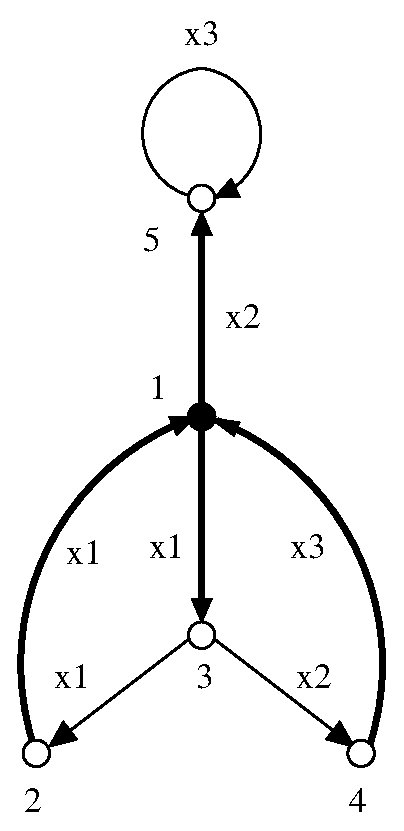
\includegraphics[scale=.52]{stallh1.eps}
\label{fig:stall1}}
\hspace{5mm}
\subfigure[$\G_{A_1}\times \G_{A_1}$: connected component of $(3,1)$.]{
\psfrag{a}{$(1,2)$}
\psfrag{b}{$(2,3)$}
\psfrag{c}{$(3,1)$}
\psfrag{d}{$(4,5)$}
\psfrag{e}{$(1,5)$}
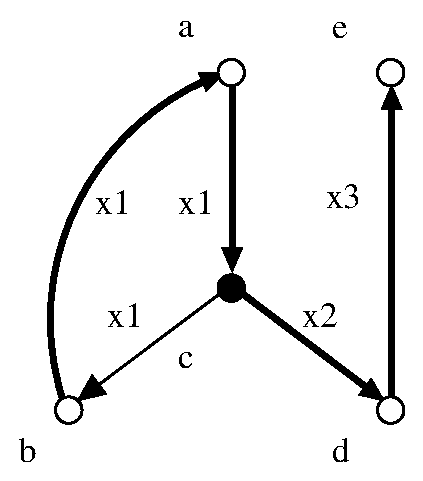
\includegraphics[scale=.52]{GxG-1.eps}
\label{fig:GxG-1}}
\hspace{5mm}
\subfigure[$\G_{A_1}\times \G_{A_1}$: connected component of $(2,1)$.]{
\psfrag{a}{$(2,1)$}
\psfrag{b}{$(3,2)$}
\psfrag{c}{$(1,3)$}
\psfrag{d}{$(5,4)$}
\psfrag{e}{$(5,1)$}
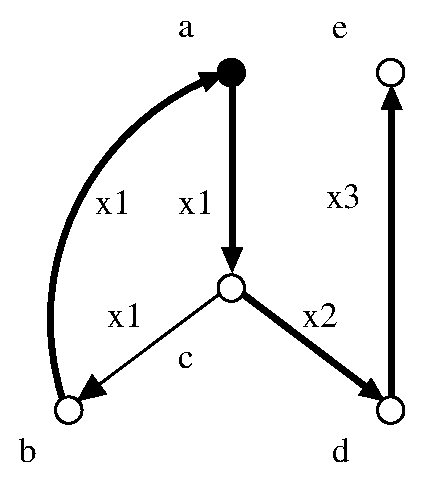
\includegraphics[scale=.52]{GxG-2.eps}
\label{fig:GxG-2}}
\end{center}
\caption{Example \ref{ex:f_1}.}\label{fig:stall}
\end{figure}

\begin{example}\label{ex:f_2}
Let $F_2$ be the free group on generators
$y_1,y_2,y_3,y_4$ with a subgroup $H_2 = \la h_1^{\prime},
h_2^{\prime},h_3^{\prime}\ra$, where
$h_1^{\prime}=y_2^2$,
$h_2^{\prime}=y_3y_4$ and
$h_3^{\prime}=y_1^2y_3y_1^{-1}y_2$.
The Stallings automata, $\G_{A_2}$ for $H_2$,
with maximal subtree $T_2$ highlighted and base vertex $1$, is shown
in Figure \ref{fig:stallagain}.\ref{fig:stallh2}.
The set $L_{T_2}$ corresponding to the maximal subtree  $T_2$ is
 $L_{T_2}=
\{1, y_1, y_1^2,
y_2^{-1}, y_2^{-1}y_1, y_3 \}$.
Let the set of double coset representatives for $H_2$ be $S_2=S_2^{(1)}
\cup S_2^{(2)}$.

To find the normal form of $f_3=y_1^2y_3y_1^{-1}y_2y_3y_4y_1y_2
y_3y_4y_2^2$: use ${A_2}$ to read off the maximal acceptable
prefix $h= y_1^2y_3y_1^{-1}y_2y_3y_4$ of $f_3$; and  the maximal
$L_{Q_2}$-prefix $p=y_1$ of the rest of $f_3$.  Next $q^{-1}=
y_2^{-2}y_4^{-1}y_3^{-1}y_2^{-1}$, so $g=y_2^{-2}y_4^{-1}y_3^{-1}$
and $t=y_2^{-1}$. This element will be represented by an element
of $S_2^{(2)}$, so we need to construct $\G_{A_2}\times \G_{A_2}$.
There are $7$  non-trivial, non-diagonal components. One is shown
in Figure \ref{fig:stallagain}\ref{fig:G2xG2-1} and the remaining
six in Figure \ref{fig:G2xG2-2}. In all cases the solid vertex
corresponds to the $\sim$ representative and connecting elements
are paths in the highlighted trees. Following Algorithm I, the
normal form of $f_3$ is seen to be
\[f_3=h yz^{-1} g^{-1},\]
where $y=y_1$, $z=y_2$ and $yz^{-1}=y_1y_2^{-1}\in S_2^{(2)}$: that is
\[f_3=h^\prime_3h_2^\prime y_1y_2^{-1} (h_1^\prime)^{-1}(h_2^\prime)^{-1}.\]
\end{example}

\begin{figure}
\begin{center}

\psfrag{y1}{$y_1$}

\psfrag{y2}{$y_2$}

\psfrag{y3}{$y_3$}

\psfrag{y4}{$y_4$}
\psfrag{1}{$1$}
\psfrag{2}{$2$}
\psfrag{3}{$3$}
\psfrag{4}{$4$}
\psfrag{5}{$5$}
\psfrag{6}{$6$}
\subfigure[Stallings automaton $A_2$ for $H_2$]{
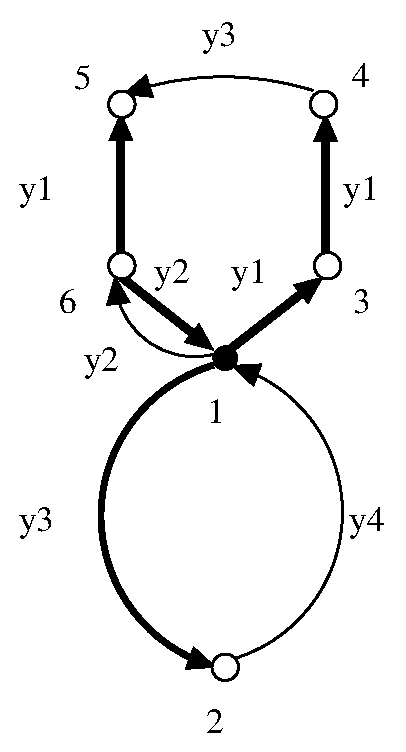
\includegraphics[scale=.52]{stallh2.eps}
\label{fig:stallh2}}
\hspace{25mm}
\subfigure[$\G_{A_2}\times \G_{A_2}$: connected component of
$(6,1)$.]{
\psfrag{a}{$(5,3)$}
\psfrag{b}{$(6,1)$}
\psfrag{c}{$(1,6)$}
\psfrag{d}{$(3,5)$}
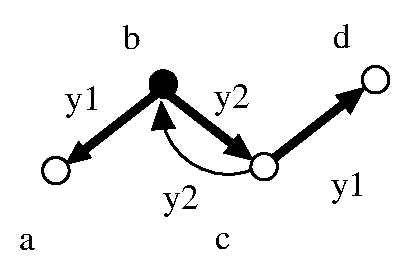
\includegraphics[scale=.52]{G2xG2-1.eps}
\label{fig:G2xG2-1}}
\end{center}
\caption{Stallings automata for Example \ref{ex:f_2}.}\label{fig:stallagain}
\end{figure}

\begin{figure}
\begin{center}

\psfrag{y1}{$y_1$}

\psfrag{y2}{$y_2$}

\psfrag{y3}{$y_3$}

\psfrag{y4}{$y_4$}
\psfrag{b}{$(1,3)$}
\psfrag{c}{$(3,4)$}
\subfigure[$(1,3)$.]{
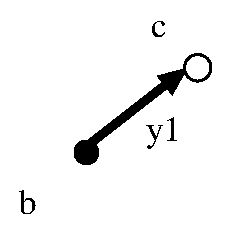
\includegraphics[scale=.5]{G2xG2-2.eps}
\label{fig:G2xG2-2-1}}
\hspace{1mm}
\subfigure[$(3,1)$.]{
\psfrag{b}{$(3,1)$}
\psfrag{c}{$(4,3)$}
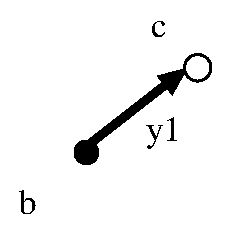
\includegraphics[scale=.5]{G2xG2-2.eps}
\label{fig:G2xG2-2-2}}
\hspace{1mm}
\subfigure[$(2,5)$.]{
\psfrag{y1}{$y_3$}
\psfrag{b}{$(1,4)$}
\psfrag{c}{$(2,5)$}
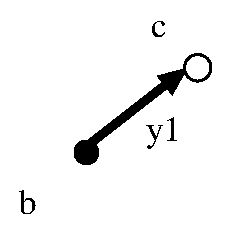
\includegraphics[scale=.5]{G2xG2-2.eps}
\label{fig:G2xG2-2-3}}
\hspace{1mm}
\subfigure[$(5,2)$.]{
\psfrag{y1}{$y_3$}
\psfrag{b}{$(4,1)$}
\psfrag{c}{$(5,2)$}
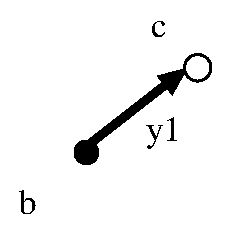
\includegraphics[scale=.5]{G2xG2-2.eps}
\label{fig:G2xG2-2-4}}
\hspace{1mm}
\subfigure[$(4,5)$.]{
\psfrag{y1}{$y_1$}
\psfrag{b}{$(3,6)$}
\psfrag{c}{$(4,5)$}
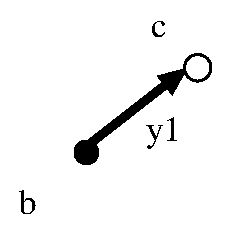
\includegraphics[scale=.5]{G2xG2-2.eps}
\label{fig:G2xG2-2-5}}
\hspace{1mm}
\subfigure[$(6,3)$.]{
\psfrag{b}{$(6,3)$}
\psfrag{c}{$(5,4)$}
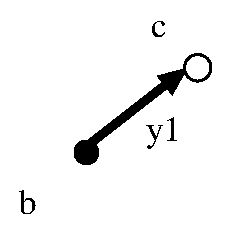
\includegraphics[scale=.5]{G2xG2-2.eps}
\label{fig:G2xG2-2-6}}
\end{center}
\caption{Example \ref{ex:f_2}: connected components of $\G_{A_2}\times \G_{A_2}$.}\label{fig:G2xG2-2}
\end{figure}